% $Header: /Users/joseph/Documents/LaTeX/beamer/solutions/conference-talks/conference-ornate-20min.en.tex,v 90e850259b8b 2007/01/28 20:48:30 tantau $
\RequirePackage{filecontents}
\begin{filecontents*}{seminar.bib}
@book{test,
author={John Smith},
title={A book},
publisher={Puplisher},
year={1742},
}
\end{filecontents*}
\documentclass{beamer}
\usepackage{graphicx}

\usepackage{latexsym}		% to get LASY symbols
\usepackage{epsfig}		% to insert PostScript figures
\usepackage{rotating}		% for sideways tables/figures
\usepackage{eufrak}
\usepackage{natbib}
\def\newblock{\hskip .11em plus .33em minus .07em}

% This file is a solution template for:

% - Talk at a conference/colloquium.
% - Talk length is about 20min.
% - Style is ornate.



% Copyright 2004 by Till Tantau <tantau@users.sourceforge.net>.
%
% In principle, this file can be redistributed and/or modified under
% the terms of the GNU Public License, version 2.
%
% However, this file is supposed to be a template to be modified
% for your own needs. For this reason, if you use this file as a
% template and not specifically distribute it as part of a another
% package/program, I grant the extra permission to freely copy and
% modify this file as you see fit and even to delete this copyright
% notice. 


\mode<presentation>
{
  \usetheme{Madrid}
  % or ...

  \setbeamercovered{transparent}
  % or whatever (possibly just delete it)
}

\documentclass{IEEEtran}
\usepackage{algpseudocode}
\usepackage[english]{babel}
% or whatever

\usepackage[latin1]{inputenc}
% or whatever

\usepackage{times}
\usepackage[T1]{fontenc}
% Or whatever. Note that the encoding and the font should match. If T1
% does not look nice, try deleting the line with the fontenc.

\newcommand{\footlineextra}[1]{\gdef\insertfootlineextra{#1}}


\newbox\footlineextrabox

% add a beamer template that sets the saved argument in a box.
% The * means that the beamer font and color "footline extra" are automatically added. 


\defbeamertemplate*{footline extra}{default}{

    \begin{beamercolorbox}[ht=2.25ex,dp=1ex,leftskip=\Gm@lmargin]{footline extra}


    \insertfootlineextra
    %\par\vspace{2.5pt}
    \end{beamercolorbox}

}

\addtobeamertemplate{footline}{%

    % set the box with the extra footline material but make it add no vertical space
    \setbox\footlineextrabox=\vbox{\usebeamertemplate*{footline extra}}


    \vskip -\ht\footlineextrabox
    \vskip -\dp\footlineextrabox

    \box\footlineextrabox%
}
{}

% patch \begin{frame} to reset the footline extra material


\let\beamer@original@frame=\frame
\def\frame{\gdef\insertfootlineextra{}\beamer@original@frame}


\footlineextra{}
\makeatother


\setbeamercolor{footline extra}{fg=structure.fg}% for instance



\title[Energy Depletion Attacks on Wireless Sensor Networks] % (optional, use only with long paper titles)
{Energy Depletion Attacks on Wireless Sensor Networks }
%
%\subtitle
%{Include Only If Paper Has a Subtitle}

\author[FARZANA.T] % (optional, use only with lots of authors)
{FARZANA.T}
% - Give the names in the same order as the appear in the paper.
% - Use the \inst{?} command only if the authors have different
%   affiliation.

\institute[MES College of Engineering] % (optional, but mostly needed)
{
 
  12MCS1004\\
  Computer Science \& Engineering\\
  Guide: Mrs.Aswathy babu}
% - Use the \inst command only if there are several affiliations.
% - Keep it simple, no one is interested in your street address.

%\date[CFP 2003] % (optional, should be abbreviation of conference name)
%{Conference on Fabulous Presentations, 2003}
% - Either use conference name or its abbreviation.
% - Not really informative to the audience, more for people (including
%   yourself) who are reading the slides online

\subject{Theoretical Computer Science}
% the beginning of each subsection:
\AtBeginSubsection[]
{
  \begin{frame}<beamer>{Outline}
    \tableofcontents[currentsection,currentsubsection]
  \end{frame}
}


% If you wish to uncover everything in a step-wise fashion, uncomment
% the following command: 

%\beamerdefaultoverlayspecification{<+->}


\begin{document}

\begin{frame}
  \titlepage
\end{frame}

%\begin{frame}{Outline}
 % \tableofcontents
  % You might wish to add the option [pausesections]
%\end{frame}


% Structuring a talk is a difficult task and the following structure
% may not be suitable. Here are some rules that apply for this
% solution: 

% - Exactly two or three sections (other than the summary).
% - At *most* three subsections per section.
% - Talk about 30s to 2min per frame. So there should be between about
%   15 and 30 frames, all told.

% - A conference audience is likely to know very little of what you
%   are going to talk about. So *simplify*!
% - In a 20min talk, getting the main ideas across is hard
%   enough. Leave out details, even if it means being less precise than
%   you think necessary.
% - If you omit details that are vital to the proof/implementation,
%   just say so once. Everybody will be happy with that.



\subsection{Introduction}
\begin{frame}{Wireless Sensor Network}
   \begin{itemize}
  \item Consists of a number of sensors spread across a geographical area. 
  \item Each sensor has wireless communication capability 
   \item Has some level of intelligence for signal processing and networking of the data
   \end{itemize}
 \end{frame} 
 

\begin{frame}{Wireless Sensor Network cntd....}  
   \begin{itemize}
  \item Sensor node has restricted power supplies, low bandwidth, small memory and limited energy. 
  \item Leads to very demanding environment to provide security. 
   \end{itemize}
 \end{frame} 

\begin{frame}{Energy Depletion Attack}
 \begin{itemize}
  \item Attacker would send data to drain a node battery and reduce network bandwidth.  
   \end{itemize}
 \end{frame} 

\subsection{Literature survey}
\begin{frame}{Literature survey}
 \begin{itemize}
  \item Wireless Sensor Network Denial of Sleep attack[1]
  \item Intrusion Tolerant routing in Wireless Sensor Network[2]
  \item Cross-Layer Design for Energy Conservation in Wireless Sensor Network[3]
   \item Energy Efficient Opportunistic Routing in Wireless Sensor Network[4] 
   \item Sleep Deprivation Attack Detection in  Wireless Sensor Network[5]
   \item Vampire Attack: Draining Life from  Wireless Sensor Network[6]
   \end{itemize}
 \end{frame} 
 
 




\begin{frame}{Vampire Attack: Draining Life from  Wireless Sensor Network[6]}
\begin{itemize}
\item Composition and transmission of a message that causes more energy to be consumed by the network.
\item Resource depletion attacks at the routing protocol layer, which permanently disable networks by quickly draining node's battery power.
\item All protocols are susceptible to Vampire attacks.
\item  Do not disrupt immediate availability, but rather work over time to entirely disable a network.
\item 2 vampire attacks: Stretch and carousel
\end{itemize}

\footlineextra{Source:  [6] Eugene Y. Vasserman, Nicholas Hopper,
 \emph{ " Vampire Attacks: Draining Life from Wireless Ad Hoc Sensor Networks"},
 IEEE transactions on mobile computing, VOL. 12, NO. 2, February 2013}
\end{frame}



\begin{frame}{Vampire Attack: Draining Life from  Wireless Sensor Network[6] cntd....}
\textbf{ Carousel attack}
\begin{itemize}
 
\item adversary composes packets with purposely introduced routing loops
\item sends packets in circles
\item allowing a single packet to repeatedly traverse the same set of nodes
 \begin{figure}[hbtp]
  \center
  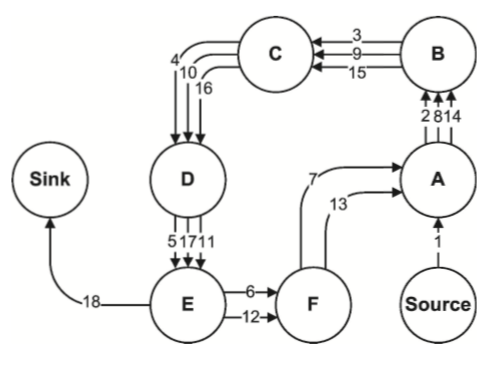
\includegraphics[scale=0.5]{cars.png}
  \caption{Carousel attack} 
  \end{figure}
\end{itemize}
\end{frame}

\begin{frame}{Vampire Attack: Draining Life from  Wireless Sensor Network[6] cntd....}
\textbf{ Stretch attack}
\begin{itemize}
 
\item An adversary constructs artificially long routes, potentially traversing every node in the network
\item Increases packet path lengths, causing packets to be processed by a number of nodes 
 \begin{figure}[hbtp]
  \center
  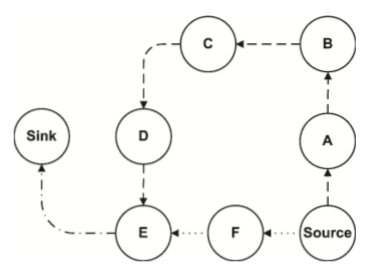
\includegraphics[scale=0.5]{strch.png}
  \caption{Stretch attack} 
  \end{figure}
\end{itemize}
\end{frame}


\begin{frame}{Vampire Attack: Draining Life from  Wireless Sensor Network[6] cntd....}
\begin{itemize}
\item Employs vampire attack on existing routing protocol PLGP.
\item PLGP:  a clean-slate secure sensor network routing protocol by B.Prano, M.Luk, E.Gustad, A.Perrig.
\item The original version of the protocol is vulnerable to Vampire attacks.
\item PLGP consists of a topology discovery phase, followed by a packet forwarding phase.

\end{itemize}
\end{frame}


\begin{frame}{Vampire Attack: Draining Life from  Wireless Sensor Network[6] cntd....}
\textbf{Discovery phase }
\begin{itemize}
\item  Deterministically organizes nodes into a tree that will later be used as an addressing scheme
\end{itemize}
\textbf{Packet forwarding}
\begin{itemize}
\item  Node determines the next hop by finding the most significant bit of its address that differs from the message originator�s address.
\end{itemize}
\end{frame} 

\begin{frame}{Vampire Attack: Draining Life from  Wireless Sensor Network[6] cntd....}
\begin{itemize}
 \begin{figure}[hbtp]
  \center
  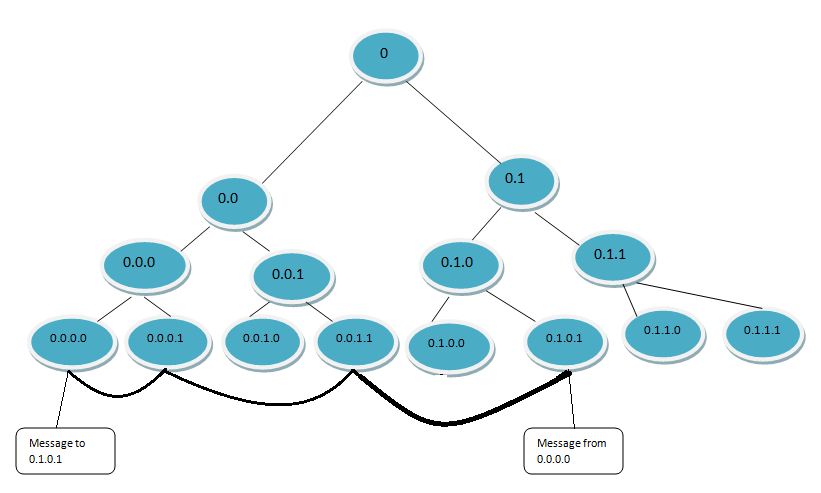
\includegraphics[scale=0.5]{btree.png}
 
  \end{figure}
\end{itemize}
\end{frame}






\begin{frame}{Vampire Attack: Draining Life from  Wireless Sensor Network[6] cntd....}
\begin{figure}[hbtp]
  \center
  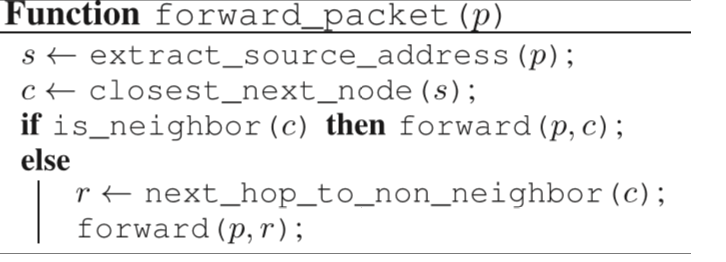
\includegraphics[scale=0.55]{frwd.png}
 
  \end{figure}
\end{frame} 

\begin{frame}{Vampire Attack: Draining Life from  Wireless Sensor Network[6] cntd....}
\begin{itemize}
\item In PLGP, forwarding nodes do not know what path a packet took.
\item Allowing adversaries to divert packets to any part of the network.
\item Makes PLGP vulnerable to Vampire attacks
\end{itemize}
\end{frame}



\begin{frame}{Vampire Attack: Draining Life from  Wireless Sensor Network[6] cntd....}
\textbf{Provable Security against Vampire Attacks}
\begin{itemize}
\item Proposed PLGP with attestations (PLGPa).
\item Add a verifiable path history to every PLGP packet.
\item PLGP with attestations (PLGPa) uses this packet history together with PLGP�s tree routing structure.
\item Every node can securely verify progress.
\item Preventing any significant adversarial influence on the path taken by any packet which traverses at least one honest node.
 
\end{itemize}
\end{frame}



\begin{frame}{Vampire Attack: Draining Life from  Wireless Sensor Network[6] cntd....}
 \begin{figure}[hbtp]
  \center
  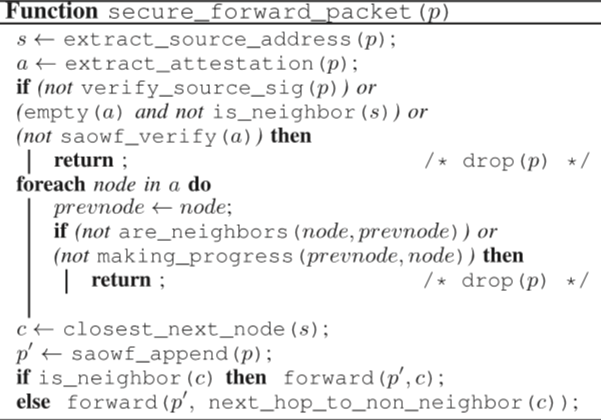
\includegraphics[scale=0.5]{plgpa.png}
  \end{figure}
\end{frame}


 \subsection{Problem Definition}
\begin{frame}{Problem Definition}
\begin{itemize}
\item  PLGPa includes path attestation increasing the size of every packet,incurring penalties in terms of bandwidth use, and thus radio power.
\item  Adding extra packet verification requirements for intermediate node increases processor utilization.
\item  Energy expenditure for cryptographic operations at intermediate hop is much greater than transmit or receive overhead.
\item  Only packet transmission phase is avoided from vampire attack, route discovery phase is not considered.
\item  Only  PLGP is considered,how the proposed solution works in other routing protocol is not considered.
\end{itemize}
\end{frame} 

\begin{frame}{concept}


\textbf{A--->B--->C--->D--->E}

\begin{itemize}
\item $ENC($(Msg)_{Prk}$,4,A)_{PrA}$== X ---> B


\item   B ----->  DEC(X)_{PB}  --->$ ENC(X,3,AB)_{PrB}$ == Y --->C


\item C -----> DEC(Y)_{PC} ---> $ENC(Y,2,ABC)_{PrC}$ == Z --> D


\item D -----> DEC(Z)_{PD}---> $ENC(Z,1,ABCD)_{PrD}$ ---->E
\end{itemize}
\end{frame}



 \subsection{Conclusion}
\begin{frame}{Conclusion}
\begin{itemize}
\item  PLGPa is not vulnerable to Vampire attacks during the forwarding phase
\item  Overhead is the main problem of this method.
\item  Can reduce overhead, use single cryptographic function instead of onion encryption.
\end{itemize}
\end{frame}

 \subsection{References}
\begin{frame}
\frametitle{References}
\footnotesize{
\begin{thebibliography}{99}



\bibitem[Label1, 2011]{key1}[1] Michael Brownfield,Yatharth Gupta,
 \newblock "Wireless Sensor Network Denial of Sleep Attack",
 \newblock \emph{Proceedings of 2005 IEEE workshop on information assurance,June 2005}.

 
  \bibitem[Label1, 2011]{key2}[2] Jing Deng, Richard Han, Shivakanth mishra,
 \newblock "INSENS: Intrusion-Tolerant routing in Wireless Sensor Networks",
 \newblock \emph{University of Colorado,Department of computer science Technical report,June 2006 }.

\bibitem[Label1, 2011]{key3}[3] Fatma Bouabdullah, Nizar Bouabdullah,Raouf Bouabdullah 
 \newblock "Cross-layer Design for Energy Conservation in  Wireless Sensor Networks",
 \newblock \emph{IEEE GLOBECOM 2008,New Orleans,USA,December 2008}.
 \bibitem[Label1, 2011]{key4}[4] Xufei Mao,Shaojie Tang, Xiahua Xu,
 \newblock "Energy efficient Oppurtunistic Routing in Wireless Sensor Network
s",
 \newblock \emph{IEEE transactions on parellel and distributed systems, VOL. 12, NO. 2, February 2011 }

\bibitem[Label1, 2011]{key5}[5] Tapaliana Bhattasali,Rituparna Chaki,Sugata Sanyal
 \newblock "Sleep Deprivation Attack Detection in Wireless Sensor Networks",
 \newblock \emph{International journal of computer applications(0975-8887)vol 40- No: 15,February 2012 }
 
 \bibitem[Label1, 2011]{key6}[6] Eugene Y. Vasserman, Nicholas Hopper,
 \newblock " Vampire Attacks: Draining Life from Wireless Ad Hoc Sensor Networks",
 \newblock \emph{IEEE transactions on mobile computing, VOL. 12, NO. 2, February 2013 }
 
  \bibitem[Label1, 2011]{key7}[7] Yazeed Al-Obaisat,Robin Braun,
 \newblock "On Wireless Sensor Networks: Architectures,Protocols,Applications and Management",
 \newblock \emph{Institute of Information and Communication Technologies,May 2004 }
  
\end{thebibliography}
}
\end{frame}

 
\begin{frame}
\centerline{Thank You}
\end{frame}
% End of slides

\end{document}

